\documentclass{article}

\usepackage[utf8]{inputenc}
\usepackage[a4paper, total={6.3in, 8.8in}]{geometry}
\usepackage{amsmath}
\usepackage{bm}
\usepackage{amsfonts}
\usepackage{graphicx}
\usepackage{amssymb}  % assumes amsmath package installed
\usepackage{graphics} % for pdf, bitmapped graphics files
\usepackage{caption}
\usepackage{subcaption}
\usepackage{todonotes}
\usepackage{titling}
\newcommand{\subtitle}[1]{%
  \posttitle{%
    \par\end{center}
    \begin{center}\large#1\end{center}
    \vskip0.5em}%
}


\title{Exercise Session 1: Classification}
\subtitle{Support Vector Machines - Final Report}
\author{Victor van Wymeersch - R0690930}
\date{May 2022}

\begin{document}

\maketitle

    % \begin{figure}
    %     \centering
    %     \includegraphics[width=0.95\textwidth]{figures/}
    %     \caption{}
    %     \label{fig:}
    % \end{figure}
    
    % \begin{figure}[h]
    %      \centering
    %      \begin{subfigure}[b]{0.8\textwidth}
    %          \centering
    %          \includegraphics[width=\textwidth]{figures/}
    %          \caption{}
    %          \label{fig:}
    %      \end{subfigure}
    %      \hfill
    %      \begin{subfigure}[b]{0.8\textwidth} 
    %          \centering
    %          \includegraphics[width=\textwidth]{figures/}
    %          \caption{}
    %          \label{fig:}
    %      \end{subfigure}
    %     \caption{}
    % \end{figure}
    
\section{Exercises}
    \subsection{Two Gaussian's}
        % Two gaussians 
        \begin{figure}
            \centering
            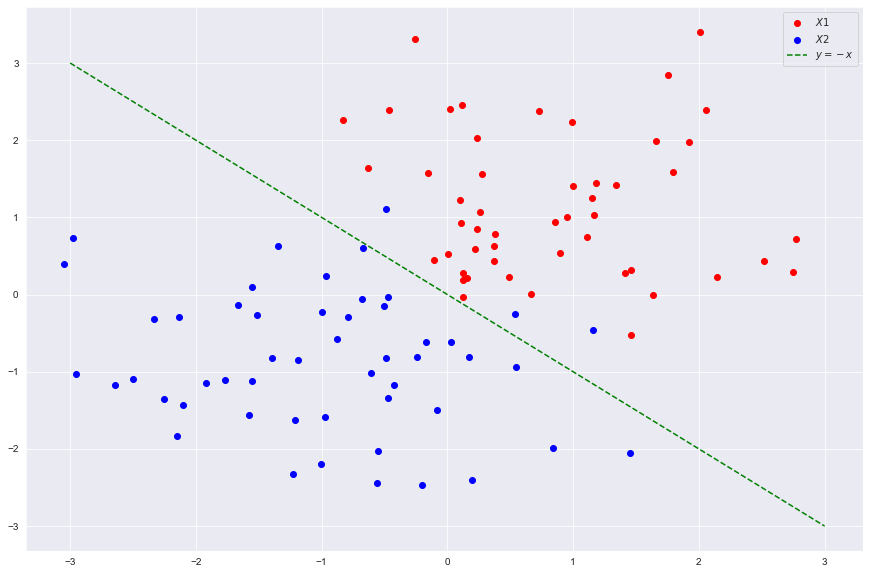
\includegraphics[width=0.60\textwidth]{Assignment 1/figures/two_gaussians.png}
            \caption{Classification boundary between two Gaussian distributions. }
            \label{fig:two_gaussians}
        \end{figure}
    
    \subsection{Support vector machine classifier}
        % Effect of number of datapoints 
        \begin{figure}[h]
             \centering
             \hspace{0.15\textwidth}
             \begin{subfigure}[b]{0.3\textwidth}
                 \centering
                 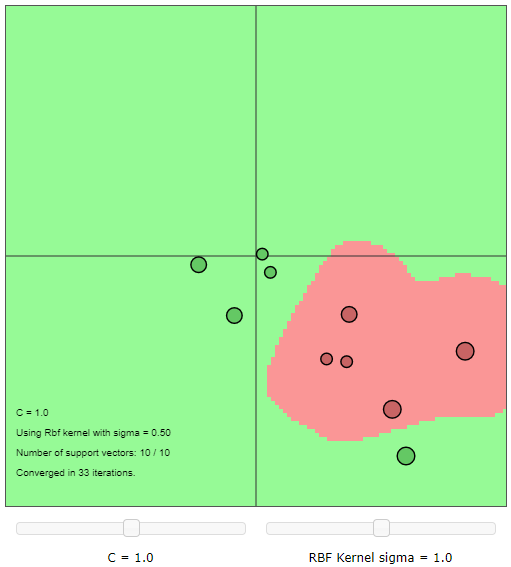
\includegraphics[width=\textwidth]{Assignment 1/figures/RBF_few_datapoints.png}
                %  \caption{Few datapoints}
                 \label{fig:few_datapoints}
             \end{subfigure}
             \hfill
             \begin{subfigure}[b]{0.3\textwidth}
                 \centering
                 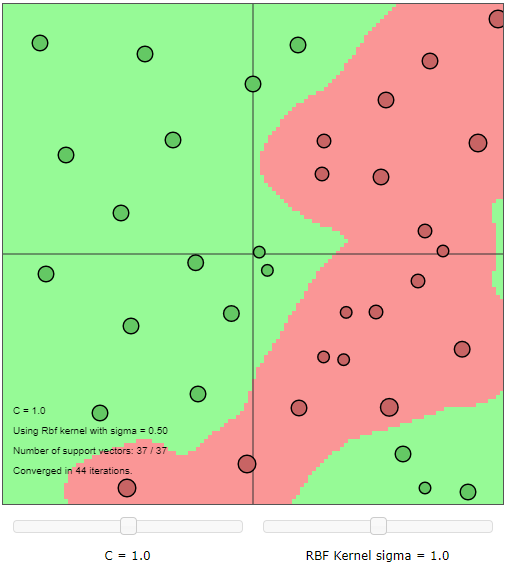
\includegraphics[width=\textwidth]{Assignment 1/figures/RBF_many_datapoints.png}
                %  \caption{Many datapoints}
                 \label{fig:many_datapoints}
             \end{subfigure}
             \hspace{0.15\textwidth}
            \caption{Effect of increasing the number of datapoints on the classification boundary.}
        \end{figure}
    
        % Effect of sigma2 values  
        \begin{figure}[h]
             \centering
             \begin{subfigure}[b]{0.3\textwidth}
                 \centering
                 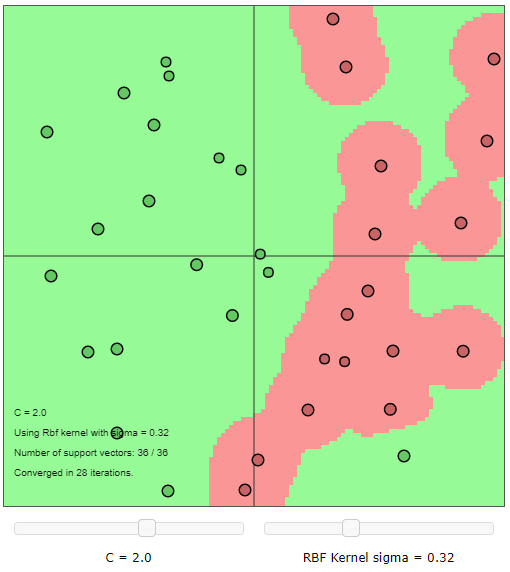
\includegraphics[width=\textwidth]{Assignment 1/figures/RBF_low_sigma.png}
                 \caption{$\sigma^2 = 0.32$}
                 \label{fig:low_sigma}
             \end{subfigure}
             \hfill
             \begin{subfigure}[b]{0.3\textwidth}
                 \centering
                 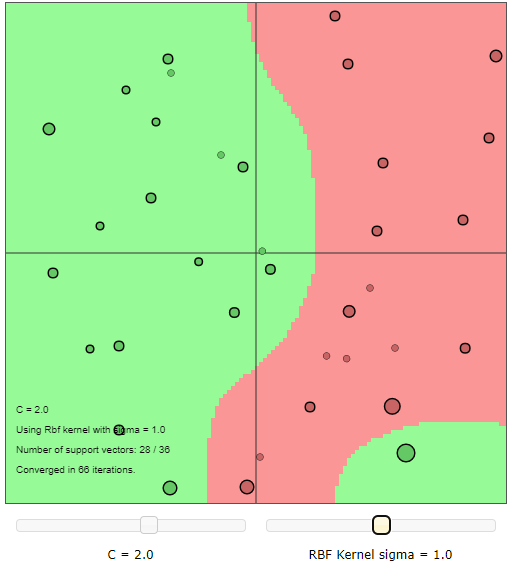
\includegraphics[width=\textwidth]{Assignment 1/figures/RBF_medium_sigma.png}
                 \caption{$\sigma^2 = 1.0$}
                 \label{fig:medium_sigma}
             \end{subfigure}
             \hfill
             \begin{subfigure}[b]{0.3\textwidth}
                 \centering
                 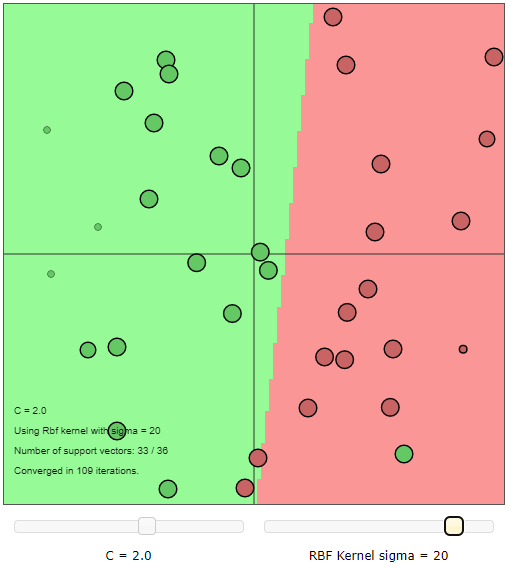
\includegraphics[width=\textwidth]{Assignment 1/figures/RBF_high_sigma.png}
                 \caption{$\sigma^2 = 20$}
                 \label{fig:high_sigma}
             \end{subfigure}
            \caption{Effect of increasing $\sigma^2$ hyperparameter on the decision boundary.}
        \end{figure}
        
        % Effect of regularisation parameter
        \begin{figure}[h]
             \centering
             \hspace{0.15\textwidth}
             \begin{subfigure}[b]{0.3\textwidth}
                 \centering
                 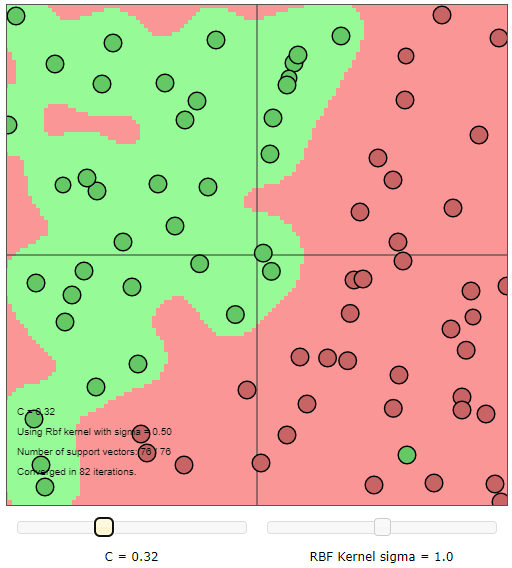
\includegraphics[width=\textwidth]{Assignment 1/figures/RBF_low_regularisation.png}
                 \caption{$C = 0.32$}
                 \label{fig:rbf_low_regularisation}
             \end{subfigure}
             \hfill
             \begin{subfigure}[b]{0.3\textwidth}
                 \centering
                 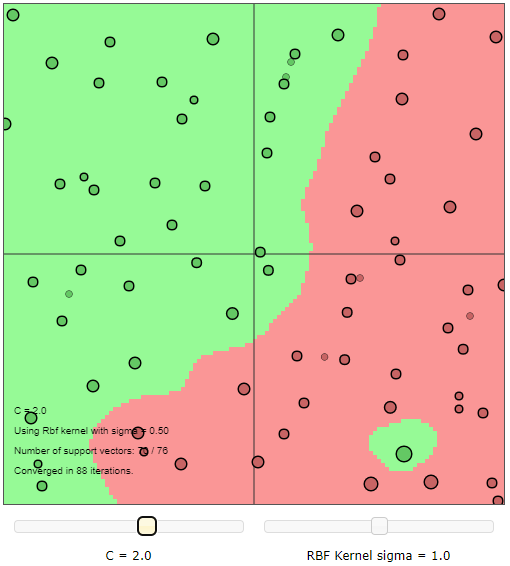
\includegraphics[width=\textwidth]{Assignment 1/figures/RBF_high_regularisation.png}
                 \caption{$C = 2$}
                 \label{fig:rbf_high_regularisation}
             \end{subfigure}
             \hspace{0.15\textwidth}
            \caption{Effect of the regularisation hyperparameter $C$ on the decision boundary.}
        \end{figure}
    
        % Linear vs RBF kernel 
        \begin{figure}[h]
             \centering
             \hspace{0.15\textwidth}
             \begin{subfigure}[b]{0.3\textwidth}
                 \centering
                 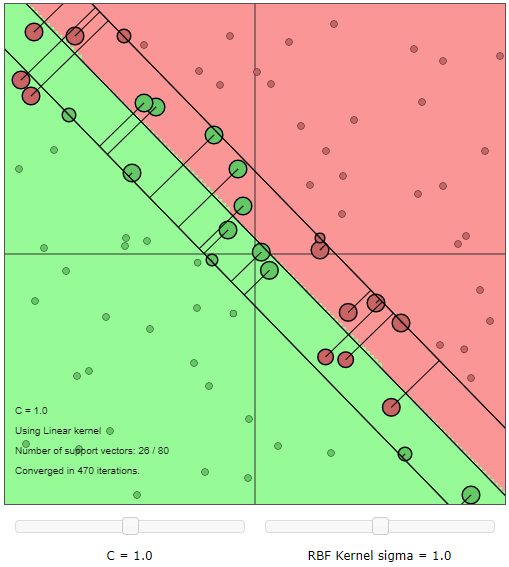
\includegraphics[width=\textwidth]{Assignment 1/figures/linear_vs_rbf_1.png}
                 \caption{Linear kernel}
                 \label{fig:linear_kernel_vs_rbf_1}
             \end{subfigure}
             \hfill
             \begin{subfigure}[b]{0.3\textwidth}
                 \centering
                 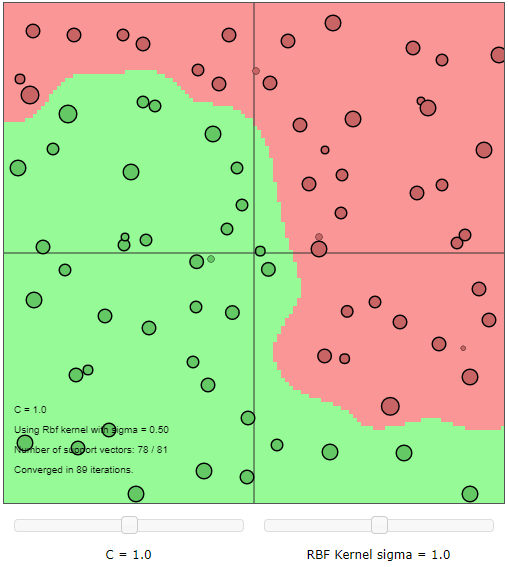
\includegraphics[width=\textwidth]{Assignment 1/figures/linear_vs_rbf_2.png}
                 \caption{RBF kernel}
                 \label{fig:linear_kernel_vs_rbf_2}
             \end{subfigure}
             \hspace{0.15\textwidth}
            \caption{Linear vs. RBF kernel classification problem. }
        \end{figure}
        
    \subsection{Least-squares support vector machine classifier}
    
        \subsubsection{Influence of hyperparameters and kernel parameters}
            
            % Effect of hyperparameters 
            \begin{figure}[h]
             \centering
             \hspace{0.05\textwidth}
             % Polynomial degree
             \begin{subfigure}[b]{0.4\textwidth}
                 \centering
                 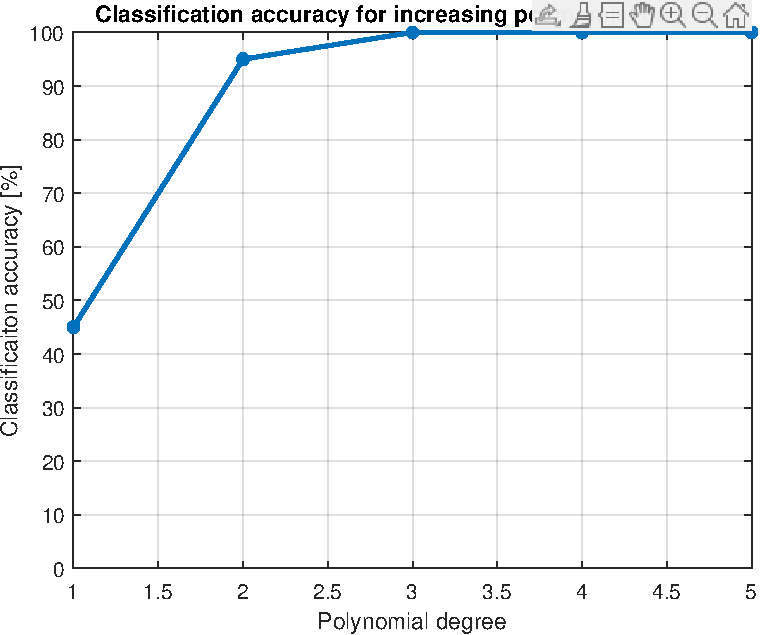
\includegraphics[width=\textwidth]{Assignment 1/figures/class_acc_poly_deg_val.pdf}
                %  \caption{Varying polynomial degree}
                 \label{fig:polynomial_degree}
             \end{subfigure}
             \hfill
             % RBF sigma2 
             \begin{subfigure}[b]{0.4\textwidth}
                 \centering
                 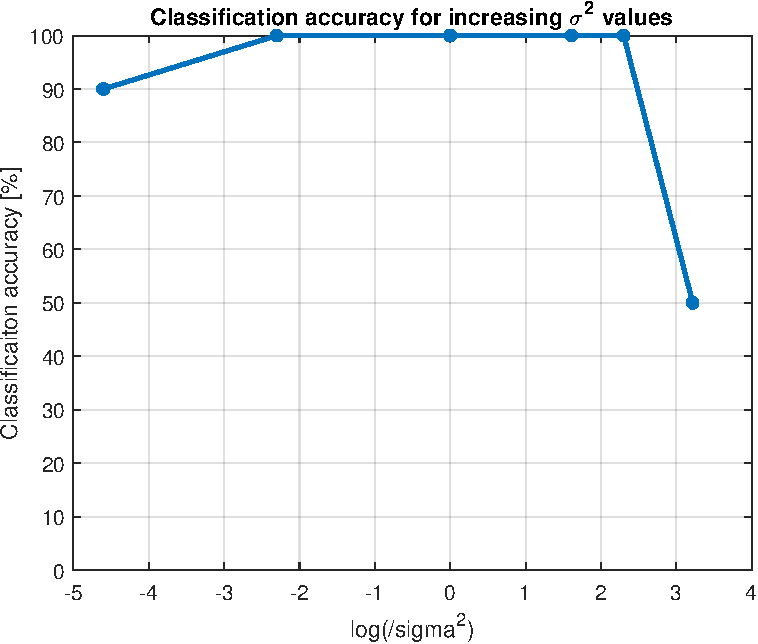
\includegraphics[width=\textwidth]{Assignment 1/figures/class_acc_sigma2_val.pdf}
                %  \caption{Varying $\sigma^2$}
                 \label{fig:rbf_sigma2}
             \end{subfigure}
             \hspace{0.05\textwidth}
            \caption{Effect of varying polynomial degree (a) and $\sigma^2$ (b) on classification accuracy. }
        \end{figure}
            
        % Tuning for Gamma and Sigma is done in the next section - just explain and point here 
            
        \subsubsection{Tuning parameters using validation}
            % Hyperparameter tuning for different validation techniques
            \begin{figure}[h]
             \centering
             \begin{subfigure}[b]{0.45\textwidth}
                 \centering
                 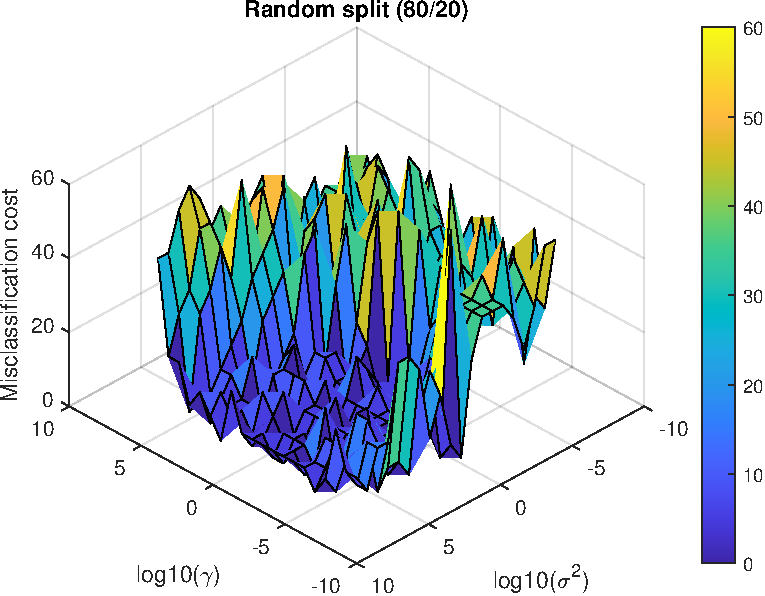
\includegraphics[width=\textwidth]{Assignment 1/figures/random_split_validation_surf.pdf}
                %  \caption{}
                 \label{fig:random_split_validation}
             \end{subfigure}
             \hfill
             \begin{subfigure}[b]{0.45\textwidth}
                 \centering
                 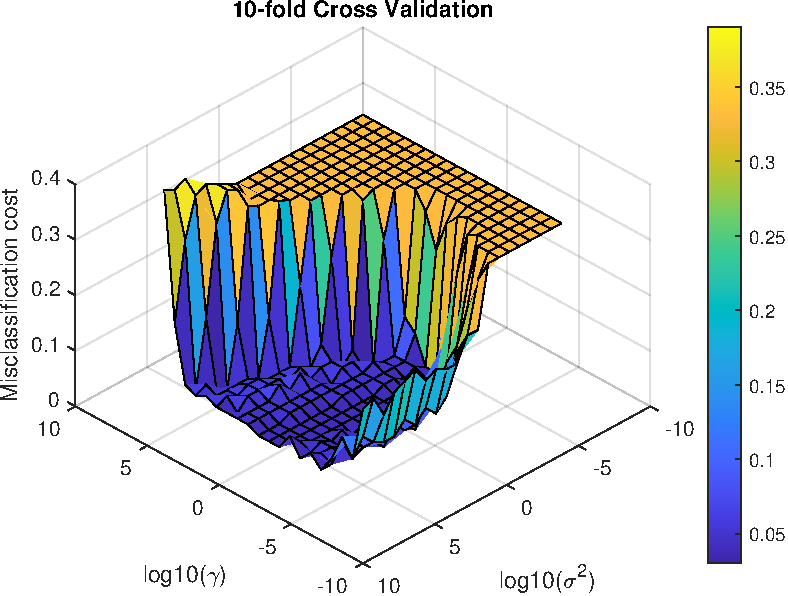
\includegraphics[width=\textwidth]{Assignment 1/figures/10_fold_cross_validation_surf.pdf}
                %  \caption{}
                 \label{fig:10_fold_validation}
             \end{subfigure}
             \hfill
             \begin{subfigure}[b]{0.45\textwidth}
                 \centering
                 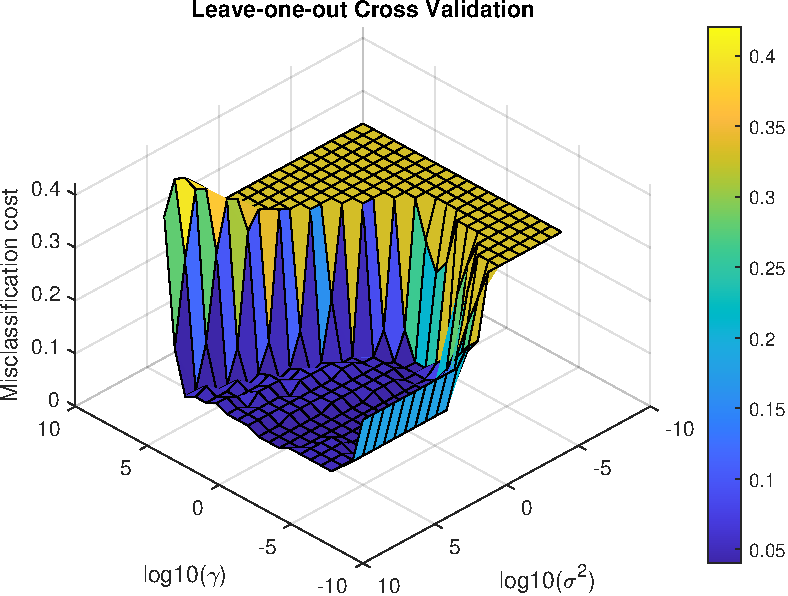
\includegraphics[width=\textwidth]{Assignment 1/figures/loo_cross_validation_surf.pdf}
                %  \caption{}
                 \label{fig:loo_validation}
             \end{subfigure}
            \caption{Effect of $\sigma^2$ and $\gamma$ hyperparameters on cost minimisation for different validation techniques. }
        \end{figure}
            
            
        \subsubsection{Automatic parameter tuning}
            % Simplex and gridsearch hyperparameter tuning results 
            \begin{figure}[h]
                 \centering
                 \hspace{0.05\textwidth}
                 % Simplex
                 \begin{subfigure}[b]{0.4\textwidth}
                     \centering
                     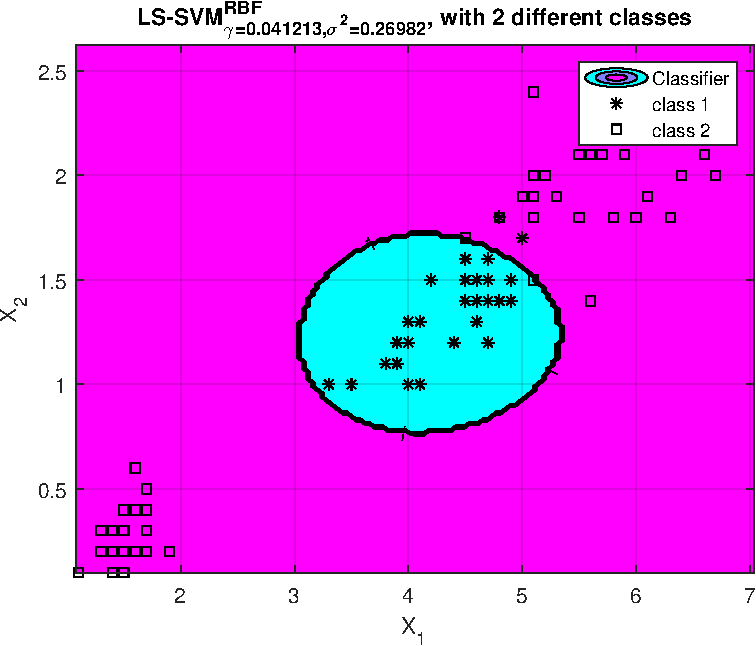
\includegraphics[width=\textwidth]{Assignment 1/figures/rbf_simplex_optimal.pdf}
                    \caption{Simplex algorithm}
                     \label{fig:rbf_simplex_tuned}
                 \end{subfigure}
                 \hfill
                 % Gridsearch
                 \begin{subfigure}[b]{0.4\textwidth}
                     \centering
                     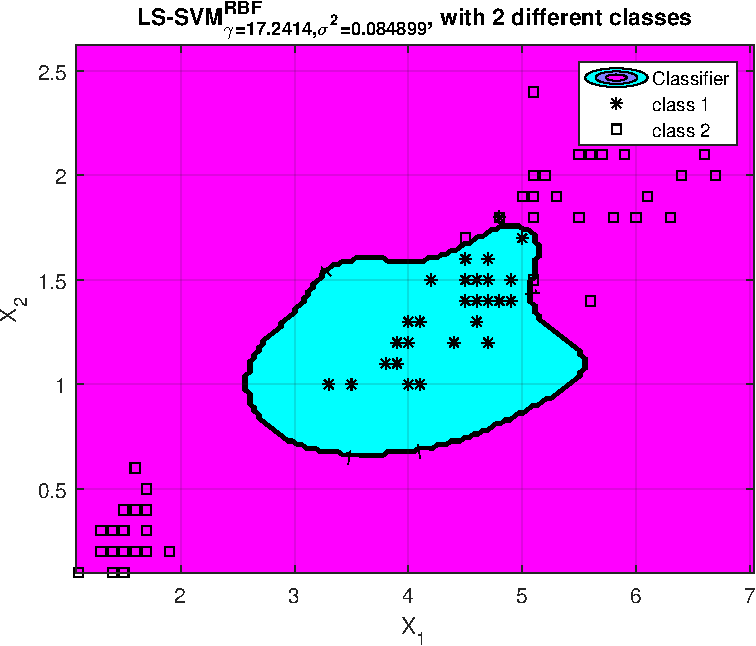
\includegraphics[width=\textwidth]{Assignment 1/figures/rbf_gridsearch_optimal.pdf}
                    \caption{Gridsearch algorithm}
                     \label{fig:rbf_gridsearch_tuned}
                 \end{subfigure}
                 \hspace{0.05\textwidth}
                \caption{Classification results for RBF kernels tuned using Simplex (a) and Gridsearch (b) algorithms.}
            \end{figure}
        
            \textbf{Simplex results:}
            \begin{itemize}
                \item $\gamma = 0.07$
                \item $\sigma^2 = 1.8$
                \item CPU time $= 2.78$
            \end{itemize}
            \textbf{Gridsearch results:}
            \begin{itemize}
                \item $\gamma = 17.24$
                \item $\sigma^2 = 0.08$
                \item CPU time $= 3.69$
            \end{itemize}
            
        \subsubsection{Using ROC curves}
             % Linear vs RBF simplex vs RBF gridsearch ROC curves
            \begin{figure}[h]
                 \centering
                 % Simplex RBF
                 \begin{subfigure}[b]{0.3\textwidth}
                     \centering
                     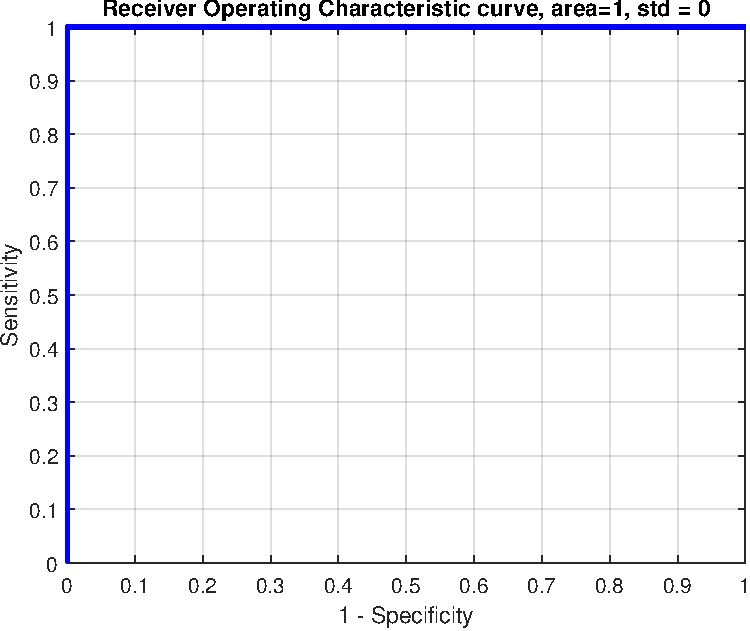
\includegraphics[width=\textwidth]{Assignment 1/figures/simplex_rbf_classifier_roc.pdf}
                    \caption{RBF Simplex}
                     \label{fig:roc_rbf_simplex_tuned}
                 \end{subfigure}
                 \hfill
                 % Gridsearch RBF
                 \begin{subfigure}[b]{0.3\textwidth}
                     \centering
                     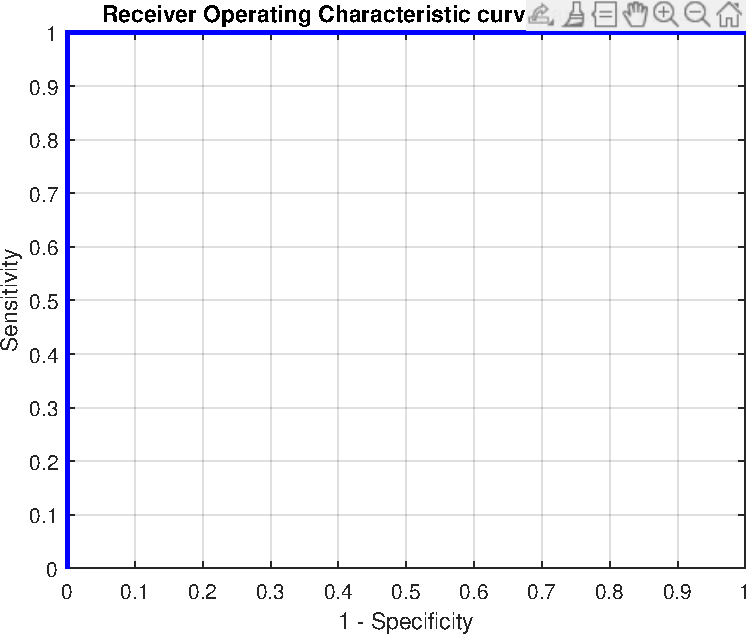
\includegraphics[width=\textwidth]{Assignment 1/figures/gridsearch_rbf_classifier_roc.pdf}
                    \caption{RBF Gridsearch}
                     \label{fig:roc_rbf_gridsearch_tuned}
                 \end{subfigure}
                 \hfill
                 % linear 
                 \begin{subfigure}[b]{0.3\textwidth}
                     \centering
                     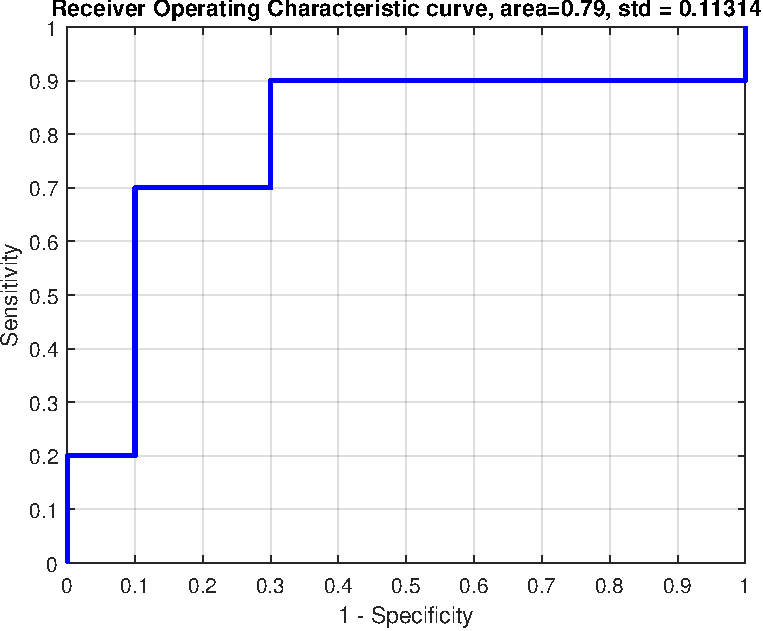
\includegraphics[width=\textwidth]{Assignment 1/figures/linear_classifier_roc.pdf}
                    \caption{Linear}
                     \label{fig:roc_linear}
                 \end{subfigure}
                \caption{ROC curves for Simplex- (a), Gridsearch-tuned RBF (b), and linear kernels (c). }
            \end{figure}
            
        
        \subsubsection{Bayesian framework} 
            % Bayesian Sigma2 tuning figures 
            \begin{figure}[h]
                 \centering
                 \begin{subfigure}[b]{0.3\textwidth}
                     \centering
                     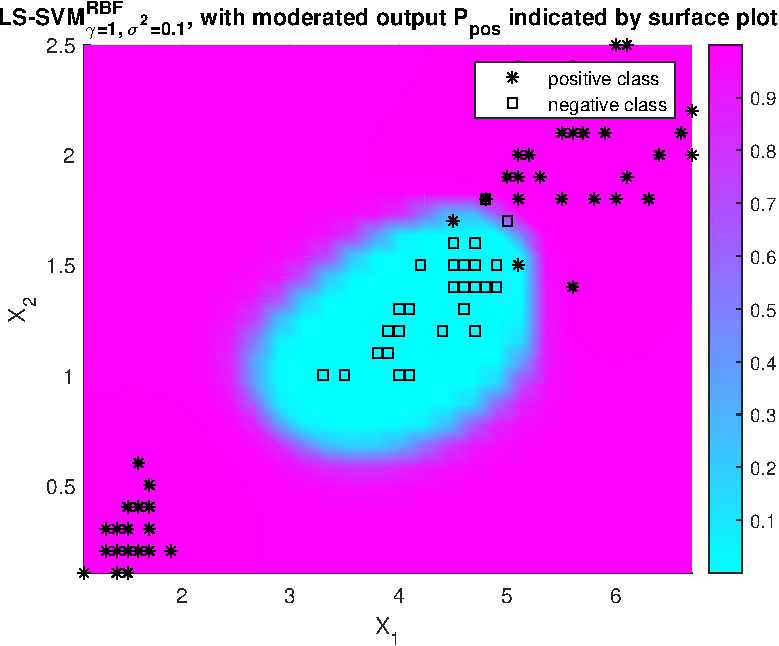
\includegraphics[width=\textwidth]{Assignment 1/figures/bayes_rbf_gamma_1_sig2_1.000000e-01}
                    \caption{$\gamma = 1,/ \sigma^2 = 0.1$}
                     \label{fig:bayes_1}
                 \end{subfigure}
                 \hfill
                 \begin{subfigure}[b]{0.3\textwidth}
                     \centering
                     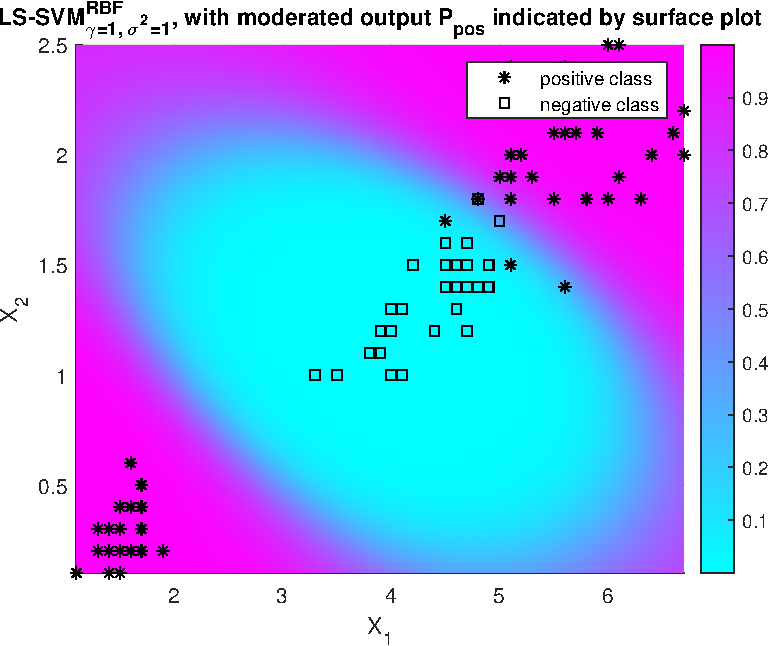
\includegraphics[width=\textwidth]{Assignment 1/figures/bayes_rbf_gamma_1_sig2_1.pdf}
                    \caption{$\gamma = 1,/ \sigma^2 = 1$}
                     \label{fig:bayes_2}
                 \end{subfigure}
                 \hfill
                 \begin{subfigure}[b]{0.3\textwidth}
                     \centering
                     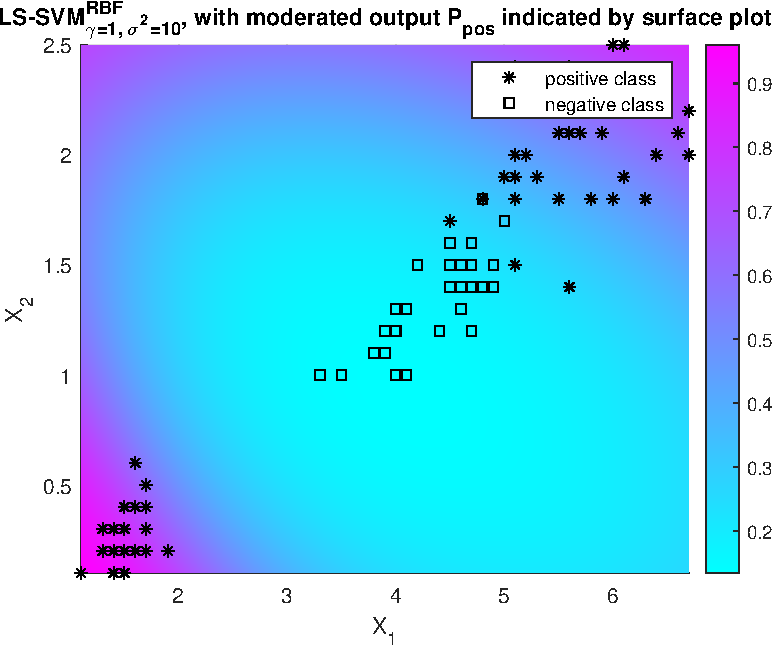
\includegraphics[width=\textwidth]{Assignment 1/figures/bayes_rbf_gamma_1_sig2_10.pdf}
                    \caption{$\gamma = 1,/ \sigma^2 = 10$}
                     \label{fig:bayes_3}
                 \end{subfigure}
                \caption{Bayesian SVM classification results for varying $\sigma^2$ values.}
            \end{figure}
            
            % Bayesian Gamma tuning figures 
            \begin{figure}[h]
                 \centering
                 \begin{subfigure}[b]{0.3\textwidth}
                     \centering
                     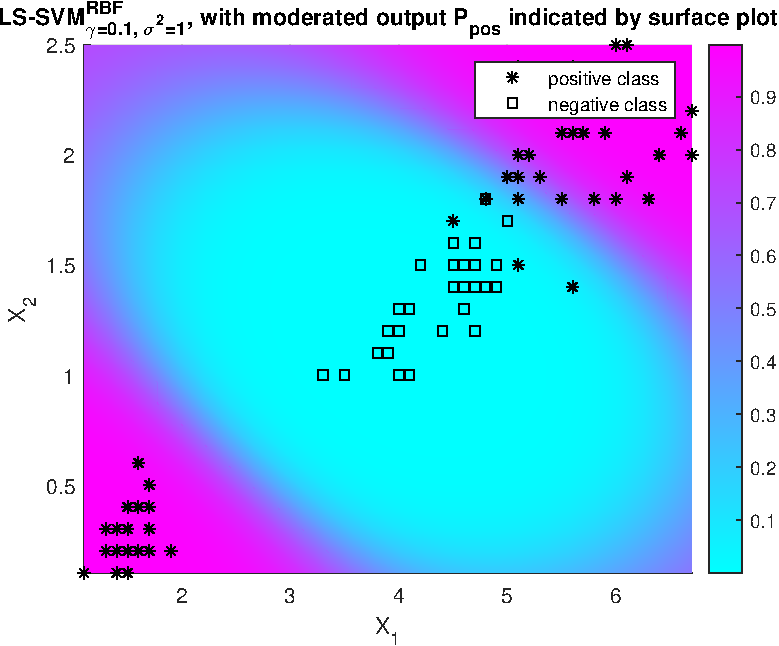
\includegraphics[width=\textwidth]{Assignment 1/figures/bayes_rbf_gamma_1.000000e-01_sig2_1.pdf}
                    \caption{$\gamma =0.01,/ \sigma^2 = 1$}
                     \label{fig:bayes_4}
                 \end{subfigure}
                 \hfill
                 \begin{subfigure}[b]{0.3\textwidth}
                     \centering
                     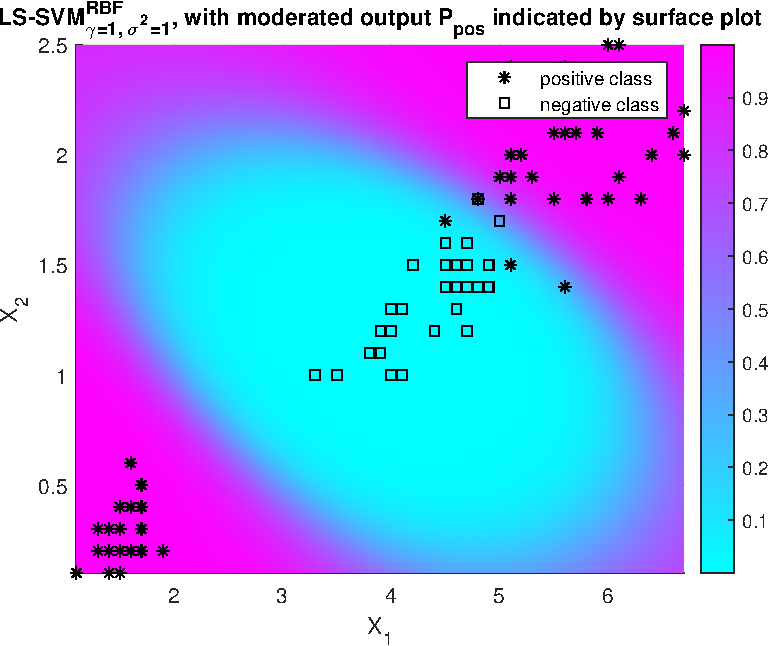
\includegraphics[width=\textwidth]{Assignment 1/figures/bayes_rbf_gamma_1_sig2_1.pdf}
                    \caption{$\gamma = 1,/ \sigma^2 = 1$}
                     \label{fig:bayes_5}
                 \end{subfigure}
                 \hfill
                 \begin{subfigure}[b]{0.3\textwidth}
                     \centering
                     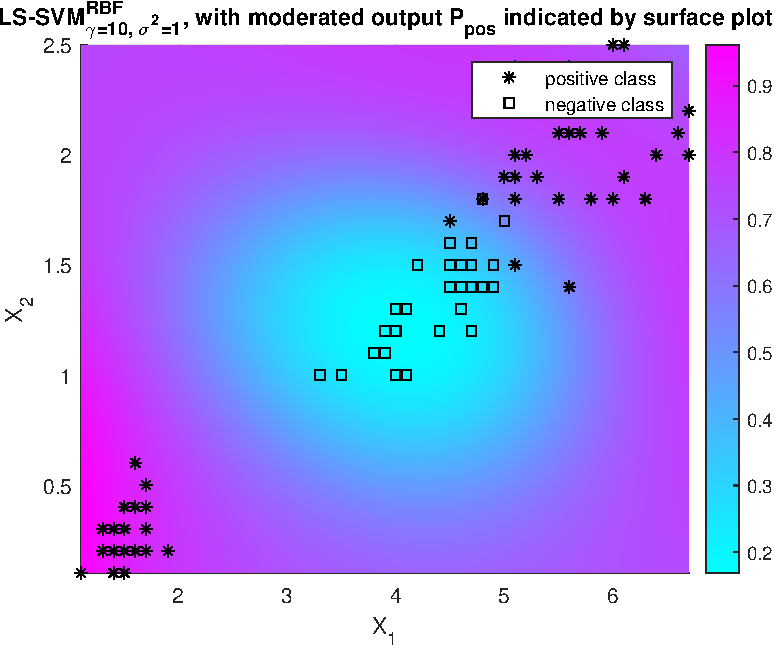
\includegraphics[width=\textwidth]{Assignment 1/figures/bayes_rbf_gamma_10_sig2_1.pdf}
                    \caption{$\gamma = 10,/ \sigma^2 = 1$}
                     \label{fig:bayes_6}
                 \end{subfigure}
                \caption{Bayesian SVM classification results for varying amounts of regularisation, $\gamma$.}
            \end{figure}
        
\section{Homework problems}
    \subsection{Ripley dataset} 
        % Ripley dataset 
        \begin{figure}
            \centering
            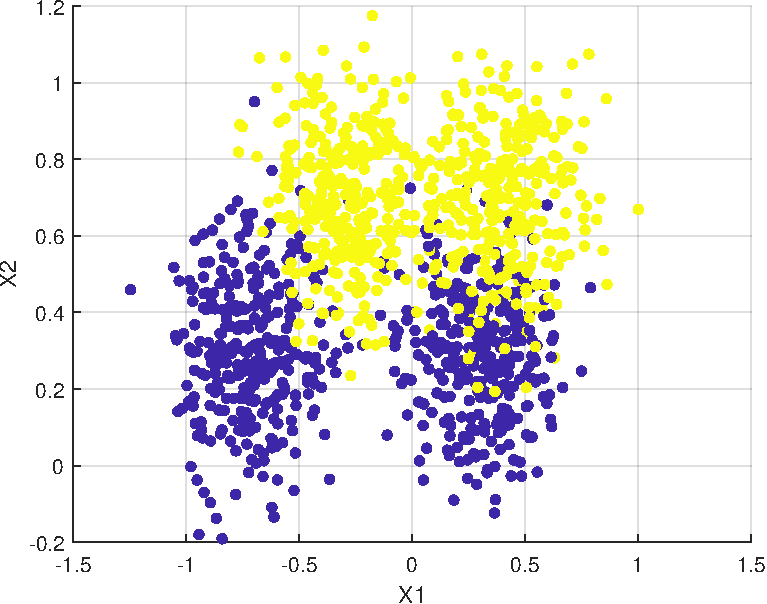
\includegraphics[width=0.60\textwidth]{Assignment 1/figures/ripley_data.pdf}
            \caption{Ripley dataset with shape $(1250,2)$, $\bar{X}_1=-0.07, \bar{X}_2=0.49$ means, and $ \sigma_1=0.48, \sigma_2=0.26$ standard deviations. }
            \label{fig:two_gaussians}
        \end{figure}
        
        % Ripley dataset for tuned Linear RBF and poly kernels 
         % Bayesian Gamma tuning figures 
            \begin{figure}[h]
                 \centering
                 \begin{subfigure}[b]{0.3\textwidth}
                     \centering
                     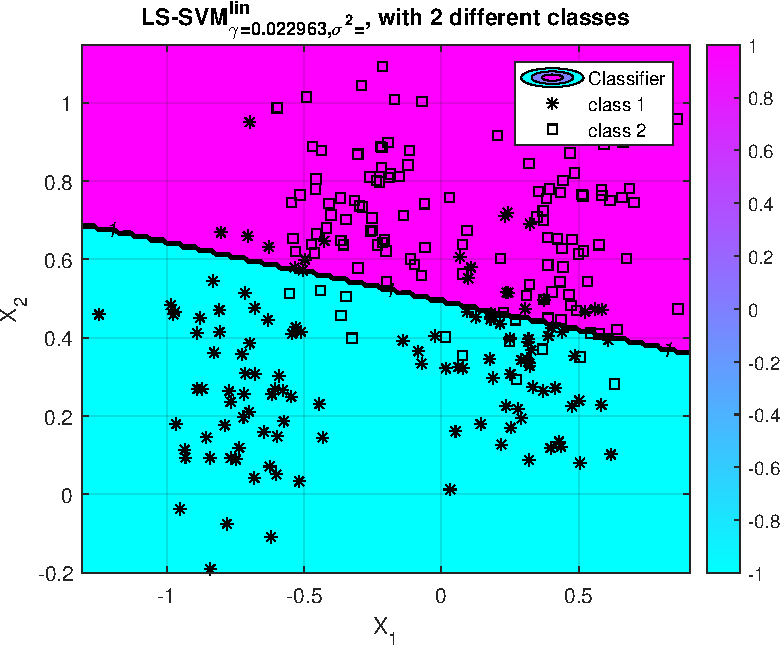
\includegraphics[width=\textwidth]{Assignment 1/figures/ripley_simplex_linear_classification_result.pdf}
                    \caption{Linear kernel}
                     \label{fig:ripley_linear_result}
                 \end{subfigure}
                 \hfill
                 \begin{subfigure}[b]{0.3\textwidth}
                     \centering
                     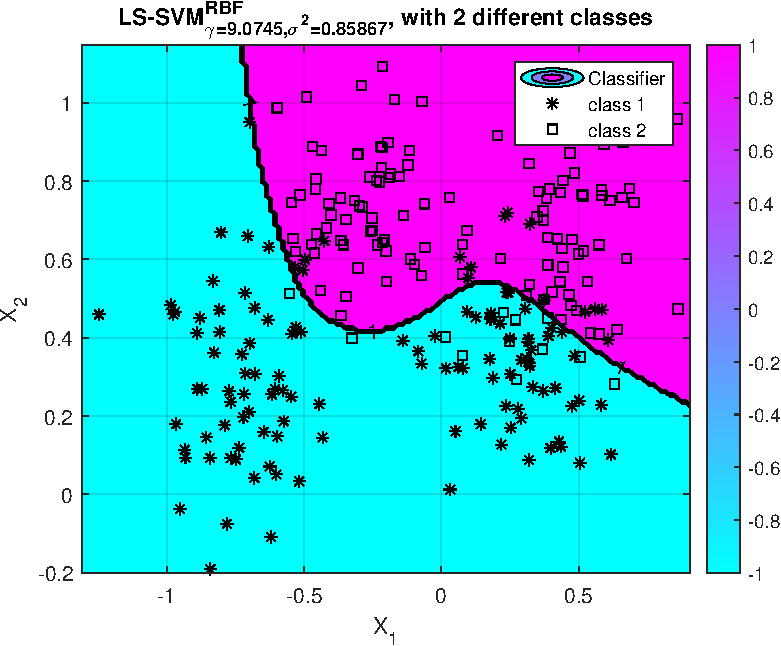
\includegraphics[width=\textwidth]{Assignment 1/figures/ripley_simplex_rbf_classification_result.pdf}
                    \caption{RBF kernel}
                     \label{fig:ripley_rbf_result}
                 \end{subfigure}
                 \hfill
                 \begin{subfigure}[b]{0.3\textwidth}
                     \centering
                     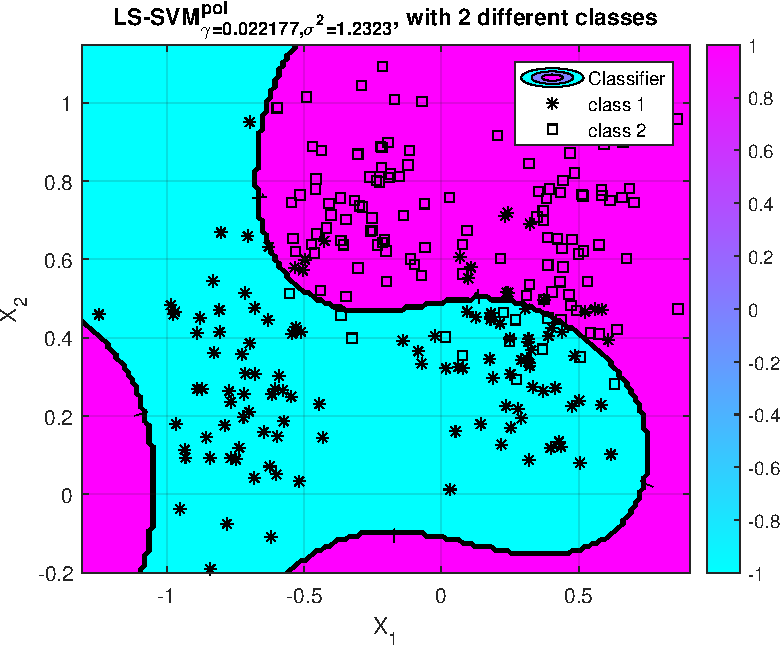
\includegraphics[width=\textwidth]{Assignment 1/figures/ripley_simplex_polynomial_classification_result.pdf}
                    \caption{Polynomial kernel}
                     \label{fig:ripley_poly_result}
                 \end{subfigure}
                 \hfill
                 \begin{subfigure}[b]{0.3\textwidth}
                     \centering
                     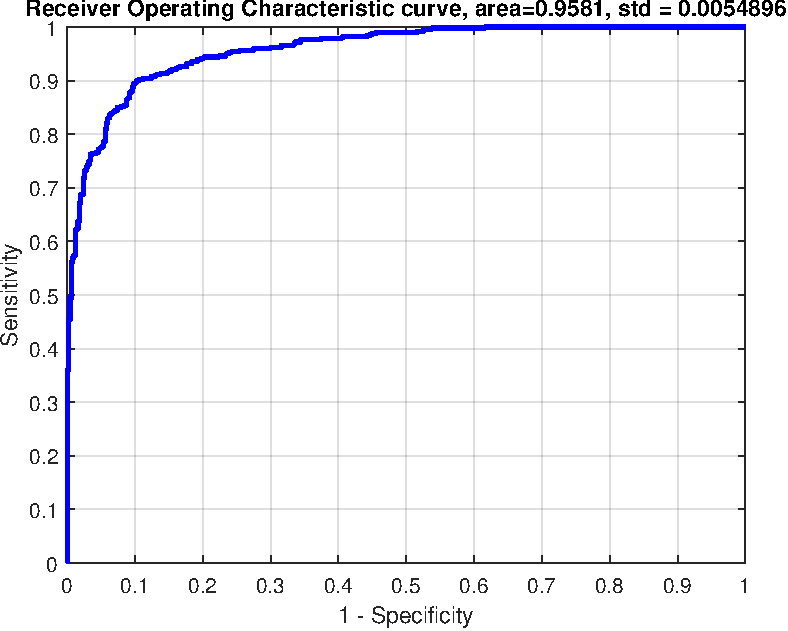
\includegraphics[width=\textwidth]{Assignment 1/figures/ripley_simplex_linear_classifier_roc.pdf}
                    \caption{Linear kernel}
                     \label{fig:ripley_linear_roc}
                 \end{subfigure}
                 \hfill
                 \begin{subfigure}[b]{0.3\textwidth}
                     \centering
                     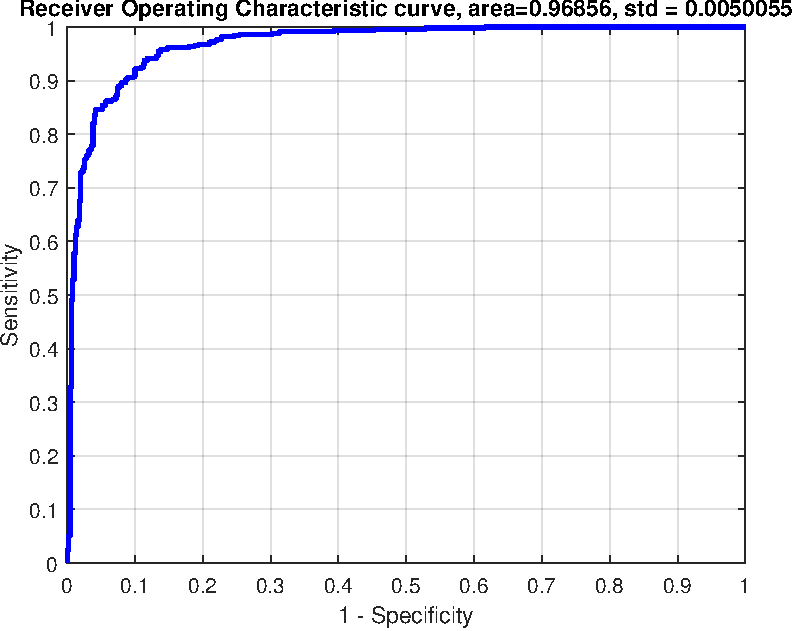
\includegraphics[width=\textwidth]{Assignment 1/figures/ripley_simplex_rbf_classifier_roc.pdf}
                    \caption{RBF kernel}
                     \label{fig:ripley_rbf_roc}
                 \end{subfigure}
                 \hfill
                 \begin{subfigure}[b]{0.3\textwidth}
                     \centering
                     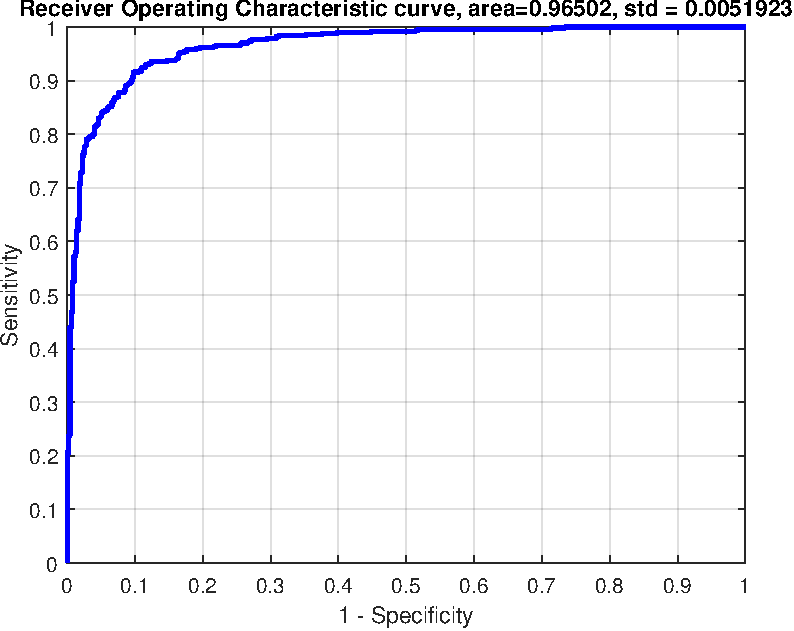
\includegraphics[width=\textwidth]{Assignment 1/figures/ripley_simplex_polynomial_classifier_roc.pdf}
                    \caption{Polynomial kernel}
                     \label{fig:ripley_poly_roc}
                 \end{subfigure}
                \caption{Classification results on the Ripley dataset for linear, RBF and Polynomial kernels tuned with the Simplex algorithm.}
            \end{figure}
        
    \subsection{Wisconsin Breast Cancer dataset}
        % Breast cancer dataset
        \begin{figure}
            \centering
            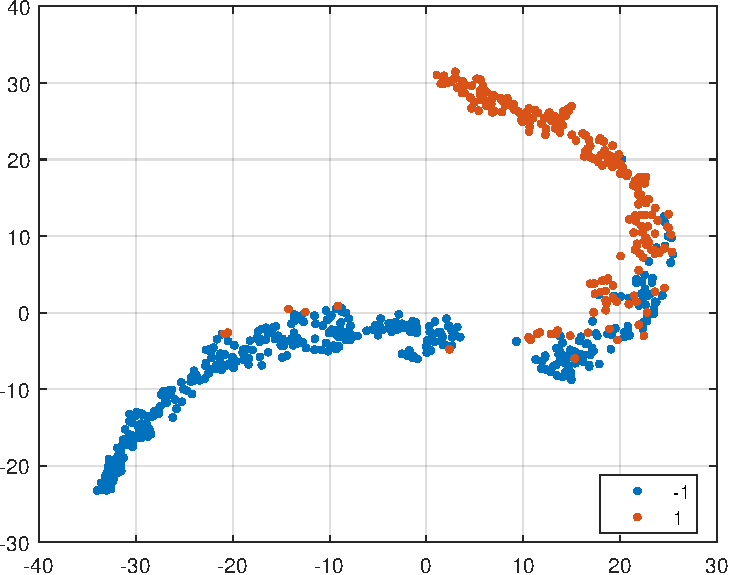
\includegraphics[width=0.60\textwidth]{Assignment 1/figures/breast_data.pdf}
            \caption{Breast cancer dataset with shape $(569,30)$.}
            \label{fig:breast_cancer_dataset}
        \end{figure}
        
        
        % ROC curves for breast cancer dataset 
        \begin{figure}[h]
             \centering
             \begin{subfigure}[b]{0.3\textwidth}
                 \centering
                 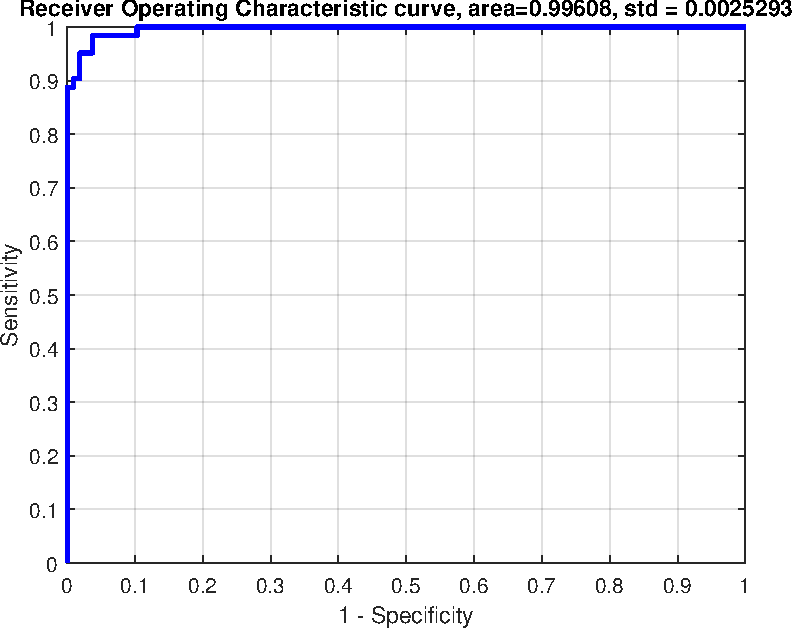
\includegraphics[width=\textwidth]{Assignment 1/figures/breast_linear_classifier_roc.pdf}
                \caption{Linear kernel}
                 \label{fig:breast_liner_roc}
             \end{subfigure}
             \hfill
             \begin{subfigure}[b]{0.3\textwidth}
                 \centering
                 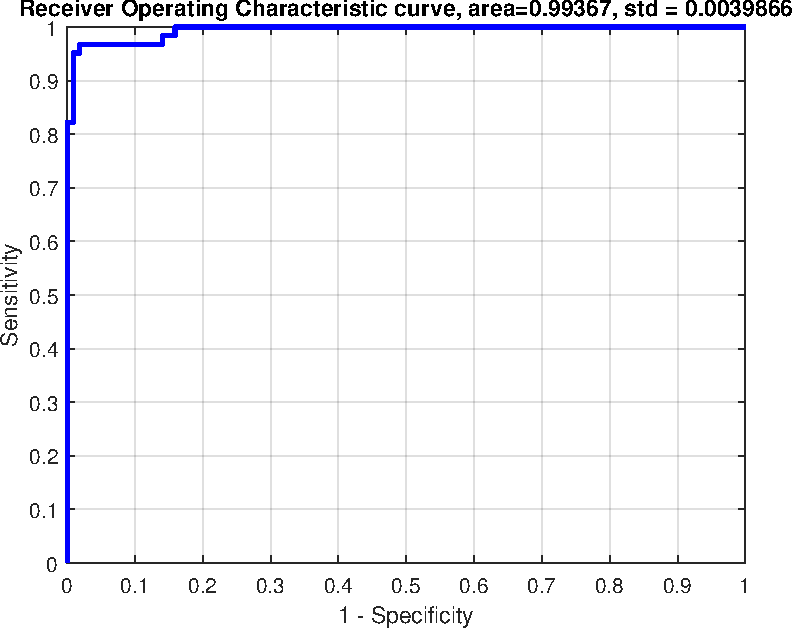
\includegraphics[width=\textwidth]{Assignment 1/figures/breast_rbf_classifier_roc.pdf}
                \caption{RBF kernel}
                 \label{fig:breast_rbf_roc}
             \end{subfigure}
             \hfill
             \begin{subfigure}[b]{0.3\textwidth}
                 \centering
                 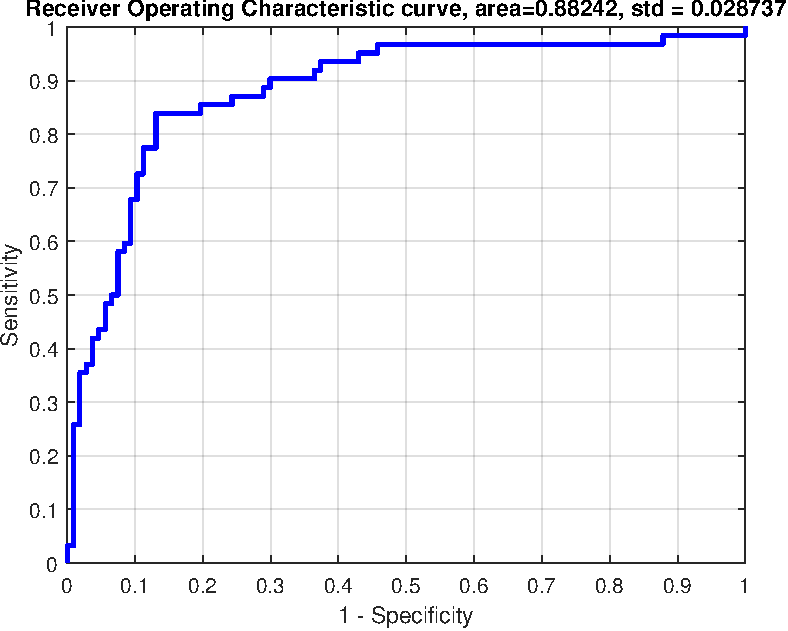
\includegraphics[width=\textwidth]{Assignment 1/figures/breast_polynomial_classifier_roc.pdf}
                \caption{Polynomial kernel}
                 \label{fig:breast_poly_roc}
             \end{subfigure}
            \caption{Binary classification results for the Breast Cancer dataset for Linear, RBF and Polynomial kernels tuned with the Simplex algorithm.}
        \end{figure}
        
    \subsection{Diabetes dataset}
        % Breast cancer dataset
        \begin{figure}
            \centering
            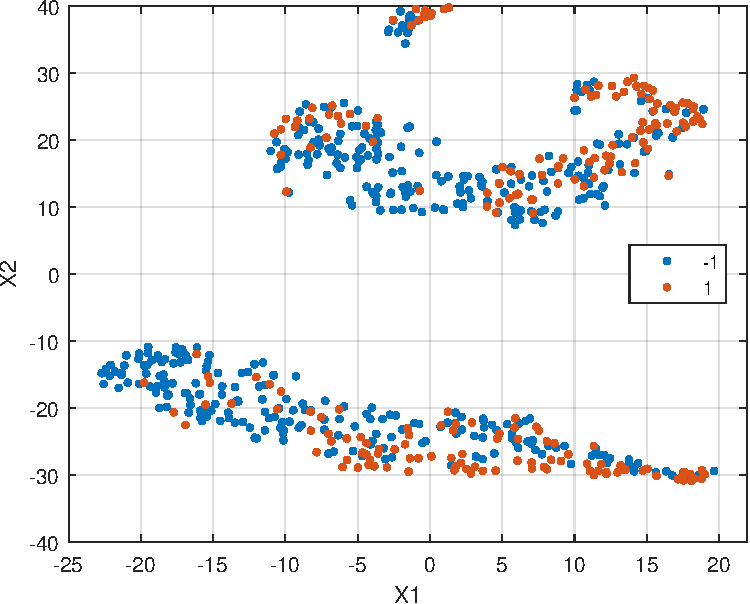
\includegraphics[width=0.60\textwidth]{Assignment 1/figures/diabetes_data.pdf}
            \caption{Diabetes dataset with shape $(600,8)$.}
            \label{fig:diabetes_dataset}
        \end{figure}
        
        % ROC curves for diabetes
        \begin{figure}[h]
             \centering
             \begin{subfigure}[b]{0.3\textwidth}
                 \centering
                 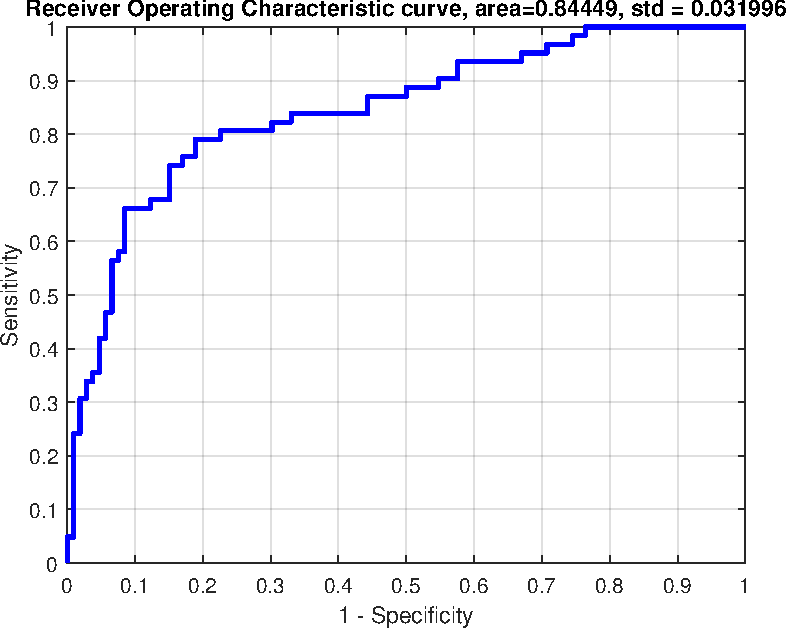
\includegraphics[width=\textwidth]{Assignment 1/figures/diabetes_linear_classifier_roc.pdf}
                \caption{Linear kernel}
                 \label{fig:diabetes_liner_roc}
             \end{subfigure}
             \hfill
             \begin{subfigure}[b]{0.3\textwidth}
                 \centering
                 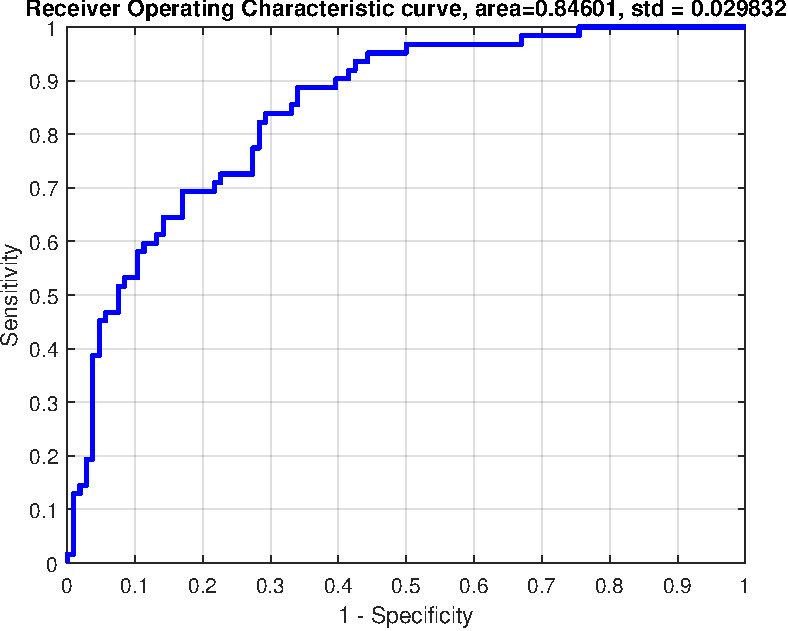
\includegraphics[width=\textwidth]{Assignment 1/figures/diabetes_rbf_classifier_roc.pdf}
                \caption{RBF kernel}
                 \label{fig:diabetes_rbf_roc}
             \end{subfigure}
             \hfill
             \begin{subfigure}[b]{0.3\textwidth}
                 \centering
                 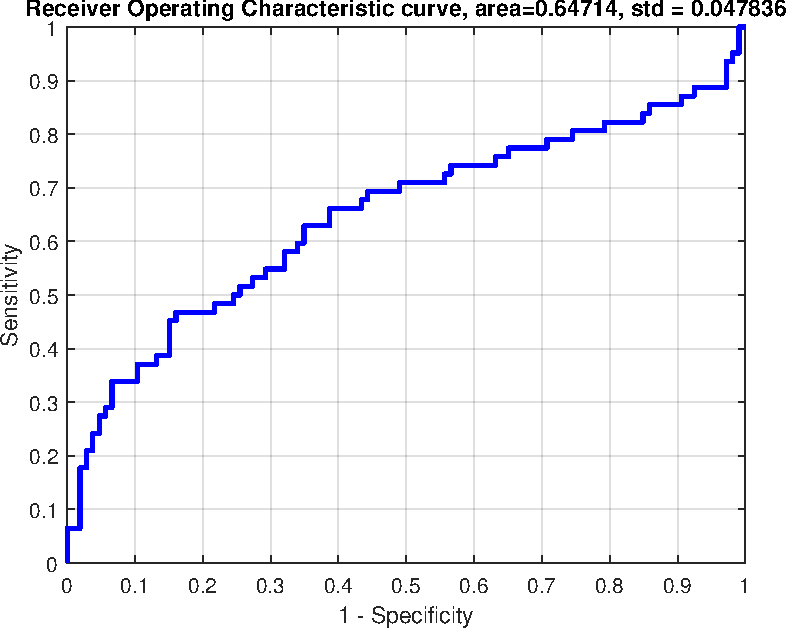
\includegraphics[width=\textwidth]{Assignment 1/figures/diabetes_polynomial_classifier_roc.pdf}
                \caption{Polynomial kernel}
                 \label{fig:diabetes_poly_roc}
             \end{subfigure}
            \caption{Binary classification results for the Diabetes dataset for Linear, RBF and Polynomial kernels tuned with the Simplex algorithm.}
        \end{figure}
        
\end{document}
